\documentclass{ximera}

%% You can put user macros here
%% However, you cannot make new environments

\listfiles

\graphicspath{{./}{firstExample/}{secondExample/}}

\usepackage{tikz}
\usepackage{tkz-euclide}
\usepackage{tikz-3dplot}
\usepackage{tikz-cd}
\usetikzlibrary{shapes.geometric}
\usetikzlibrary{arrows}
\usetikzlibrary{decorations.pathmorphing,patterns}
\usetkzobj{all}
\pgfplotsset{compat=1.13} % prevents compile error.

\renewcommand{\vec}[1]{\mathbf{#1}}
\newcommand{\RR}{\mathbb{R}}
\newcommand{\dfn}{\textit}
\newcommand{\dotp}{\cdot}
\newcommand{\id}{\text{id}}
\newcommand\norm[1]{\left\lVert#1\right\rVert}
 
\newtheorem{general}{Generalization}
\newtheorem{initprob}{Exploration Problem}

\tikzstyle geometryDiagrams=[ultra thick,color=blue!50!black]

\usepackage{mathtools}

\title{Undetermined Coefficients for Higher Order Equations}%\label{Module 7-ADEF}


\begin{document}

\begin{abstract}

\end{abstract}

\maketitle

\section*{Undetermined Coefficients for Higher Order Equations}

In this section we consider the constant coefficient equation
\begin{equation}
 \label{eq:9.3.1} a_0y^{(n)}+a_1y^{(n-1)}+\cdots+a_ny=F(x),
\end{equation}
where $n\geq 3$ and $F$ is a linear combination of
functions of the form
$$
e^{\alpha x}\left(p_0+p_1x+\cdots+p_kx^k\right)
$$
or
$$
e^{\lambda x}\left[\left(p_0+p_1x+\cdots+p_kx^k\right)
\cos\omega x+
\left(q_0+q_1x+\cdots+q_kx^k\right)
\sin\omega x\right].
$$

From Theorem~\ref{thmtype:9.1.5}, the general solution of \eqref{eq:9.3.1} is
$y=y_p+y_c$, where $y_p$ is a particular solution of \eqref{eq:9.3.1} and
$y_c$ is the general solution of the complementary equation
$$
a_0y^{(n)}+a_1y^{(n-1)}+\cdots+a_ny=0.
$$
In Section~9.2 we learned how to find $y_c$. Here
we
will learn how to find $y_p$ when the forcing function has the form stated
above. The procedure that we  use is a generalization of the
method that we used in Sections~5.4 and
5.5, and is again called
\dfn{method of undetermined coefficients}. Since
the underlying ideas are the same as those in
Sections~5.4 and 5.5,
we'll give  an informal presentation based on
examples.

\subsection*{Forcing Functions of the Form
$e^{\alpha x}\left(p_0+p_1x+\cdots+p_kx^k\right)$}

We  first consider  equations of the form
$$
a_0y^{(n)}+a_1y^{(n-1)}+\cdots+a_ny=e^{\alpha
x}\left(p_0+p_1x+\cdots+p_kx^k\right).
$$

\begin{example}\label{example:9.3.1}
Find a particular solution of
\begin{equation} \label{eq:9.3.2}
y'''+3y''+2y'-y=e^x(21+24x+28x^2+5x^3).
\end{equation}


\begin{explanation} Substituting
\begin{eqnarray*}
y&=&ue^x,\\ y'&=&e^x(u'+u),\\
y''&=&e^x(u''+2u'+u),\\
y'''&=&e^x(u'''+3u''+3u'+u)
\end{eqnarray*}
into \eqref{eq:9.3.2} and canceling $e^x$ yields
$$
(u'''+3u''+3u'+u)+3(u''+2u'+u)+2(u'+u)-u
=21+24x+28x^2+5x^3,
$$
or
\begin{equation} \label{eq:9.3.3}
u'''+6u''+11u'+5u=21+24x+28x^2+5x^3.
\end{equation}
Since the unknown $u$ appears on the left, we can see that
\eqref{eq:9.3.3} has a particular solution of the form
$$
u_p=A+Bx+Cx^2+Dx^3.
$$
Then
\begin{eqnarray*}
u_p'&=&B+2Cx+3Dx^2\\
u_p''&=&2C+6Dx\\
u_p'''&=&6D.
\end{eqnarray*}
Substituting from the last four equations  into the left side of
\eqref{eq:9.3.3} yields
\begin{eqnarray*}
u_p'''+6u_p''+11u_p'+5u_p&=&6D+6(2C+6Dx)+11(B+2Cx+3Dx^2)\\
&&+5(A+Bx+Cx^2+Dx^3)\\
&=&(5A+11B+12C+6D)+(5B+22C+36D)x\\&&+(5C+33D)x^2+5Dx^3.
\end{eqnarray*}
Comparing coefficients of like powers of $x$ on the right sides of
this equation and \eqref{eq:9.3.3} shows that $u_p$ satisfies \eqref{eq:9.3.3}
if
$$
\begin{array}{rcr}
5D&=&5\\
5C+33D&=&28\\
5B+22C+36D&=&24\\
5A+11B+12C+6D&=&21.
\end{array}
$$
Solving these equations successively yields $D=1$, $C=-1$, $B=2$, $A=1$.
Therefore
$$
u_p=1+2x-x^2+x^3
$$
is a particular solution of  \eqref{eq:9.3.3}, so
$$
y_p=e^xu_p=e^x(1+2x-x^2+x^3)
$$
is a particular solution of  \eqref{eq:9.3.2}.


\begin{image}
 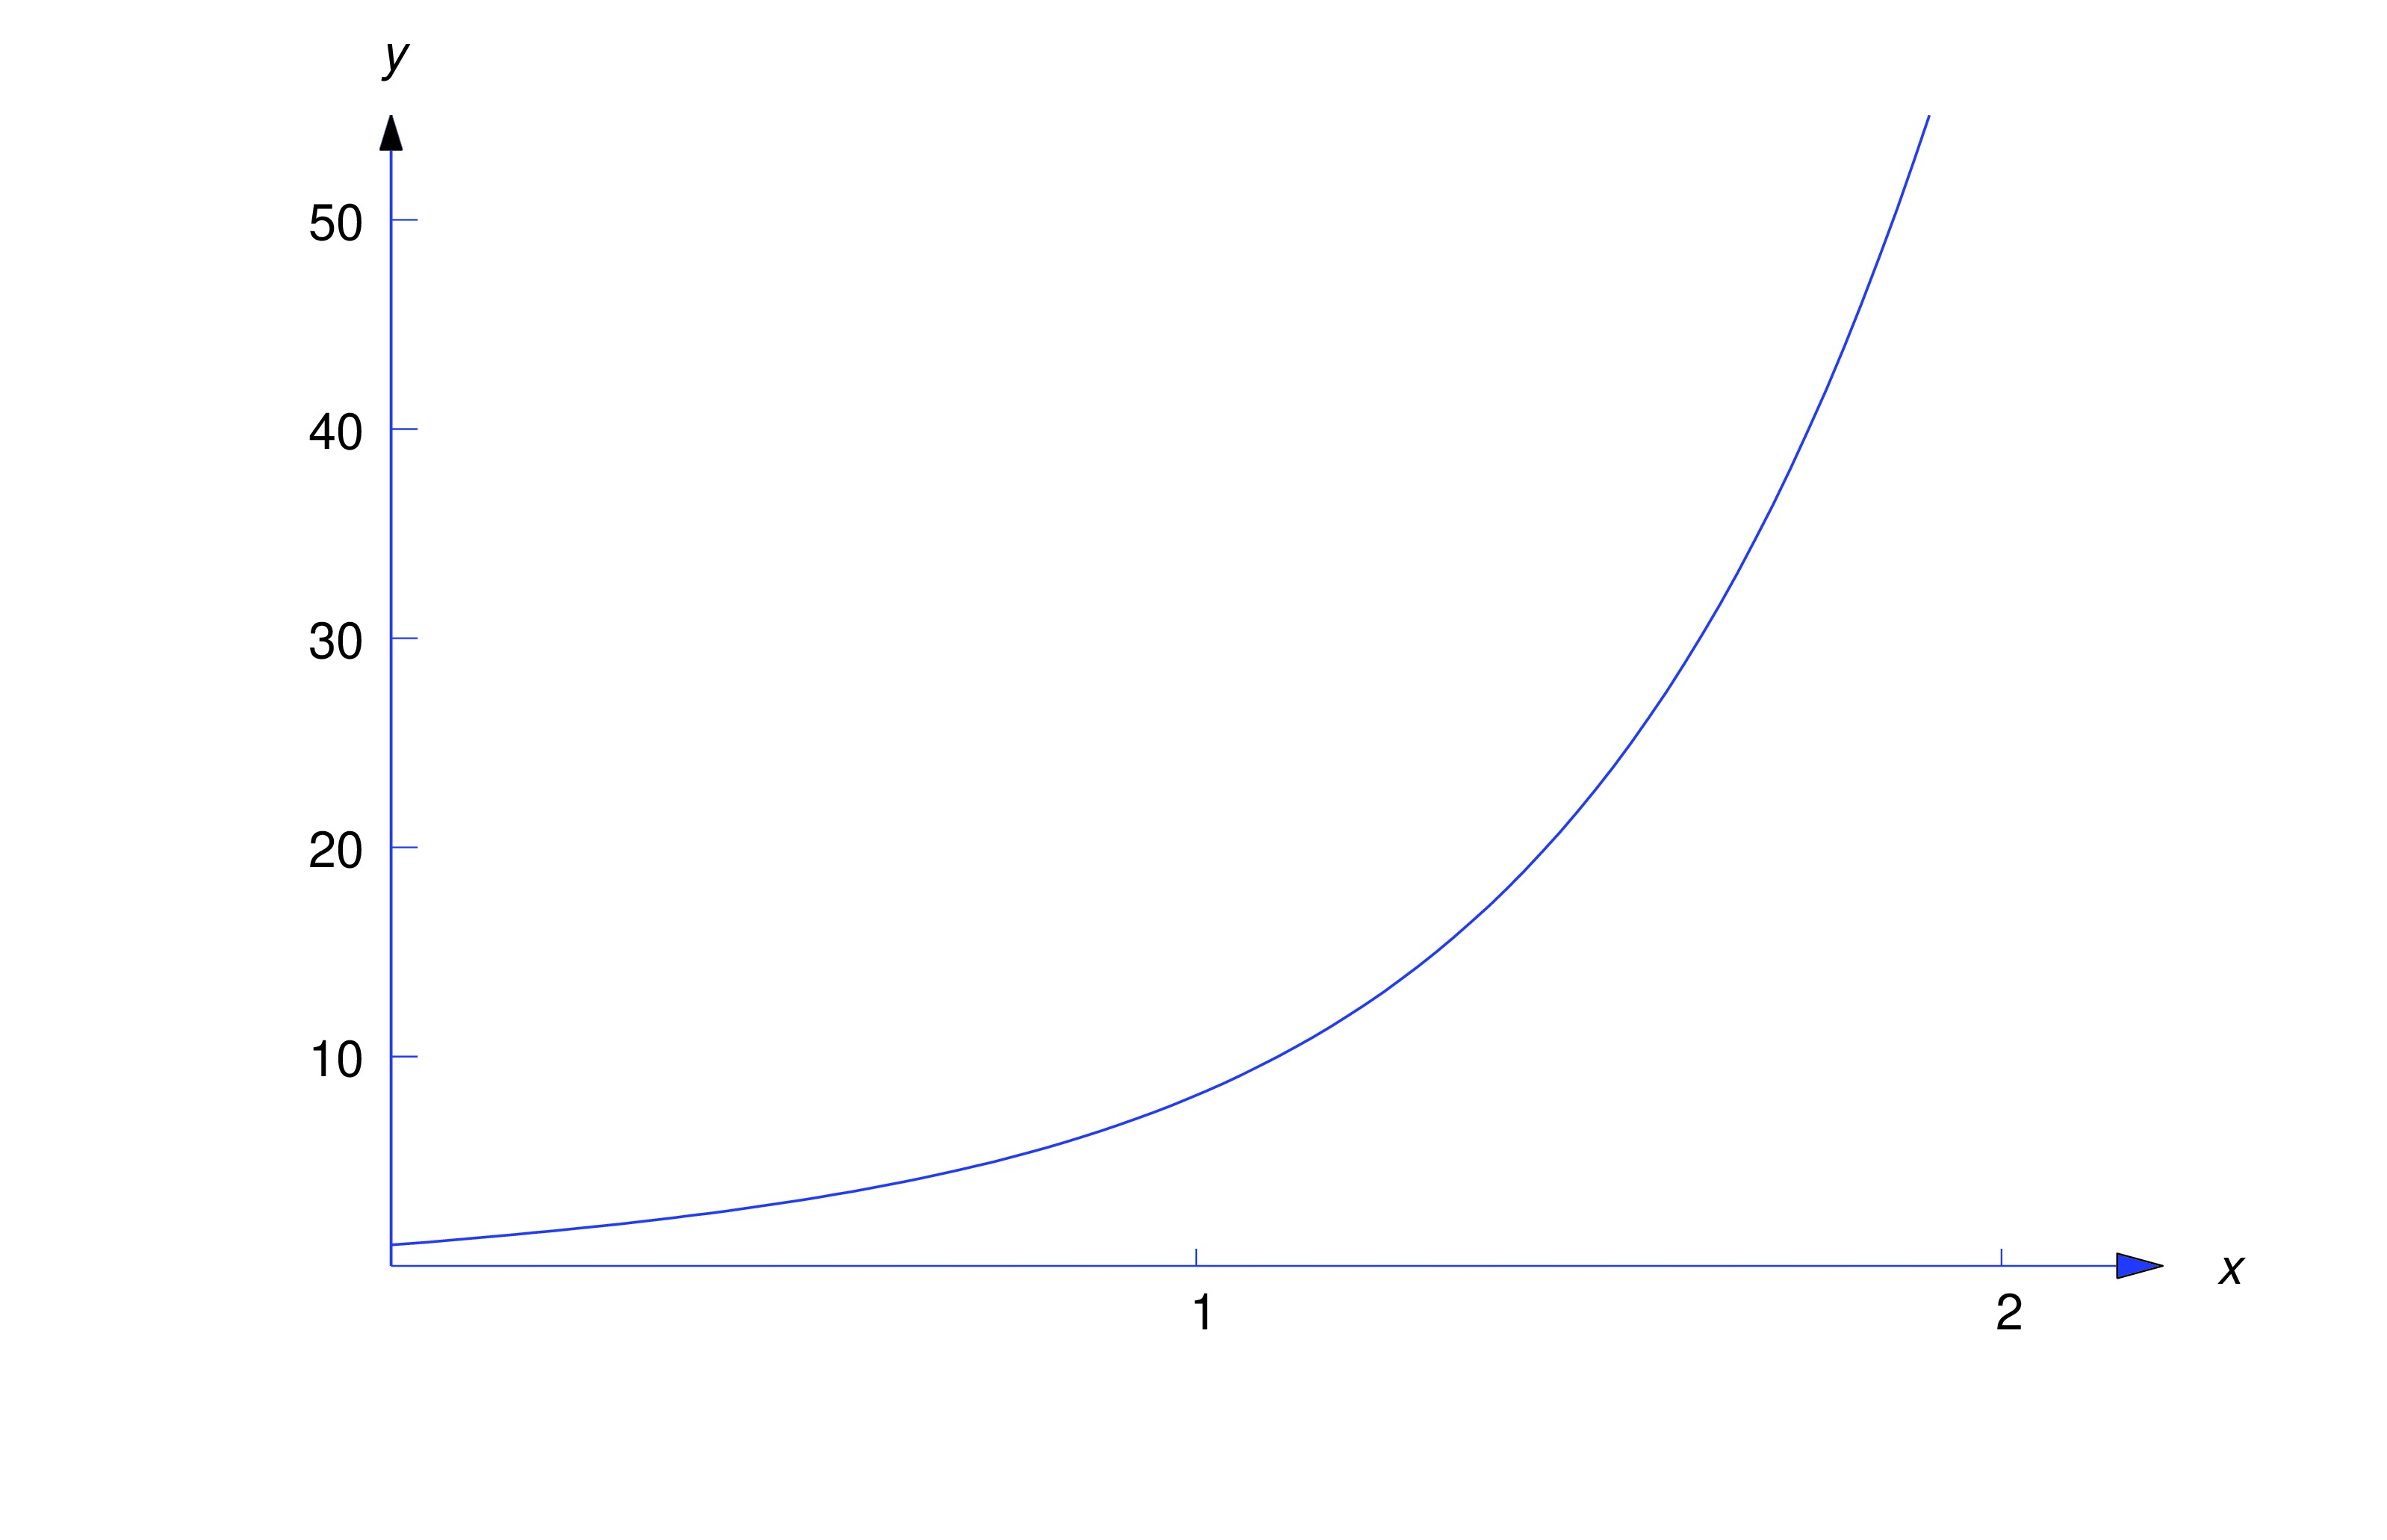
\includegraphics[height=1.5in]{fig090301.jpg} 
\end{image}

\end{explanation}
\end{example}

\begin{example}\label{example:9.3.2}
Find a particular solution of
\begin{equation} \label{eq:9.3.4}
y^{(4)}-y'''-6y''+4y'+8y=e^{2x}(4+19x+6x^2).
\end{equation}

\begin{explanation}
Substituting
\begin{eqnarray*}
y&=&ue^{2x},\\ y'&=&e^{2x}(u'+2u),\\
y''&=&e^{2x}(u''+4u'+4u),\\
y'''&=&e^{2x}(u'''+6u''+12u'+8u),\\
y^{(4)}&=&e^{2x}(u^{(4)}+8u'''+24u''+32u'+16u)
\end{eqnarray*}
into \eqref{eq:9.3.4} and canceling $e^{2x}$ yields
\begin{eqnarray*}
&&(u^{(4)}+8u'''+24u''+32u'+16u)-(u'''+6u''+12u'+8u)\\
&&-6(u''+4u'+4u)+4(u'+2u)+8u=4+19x+6x^2,
\end{eqnarray*}
or
\begin{equation} \label{eq:9.3.5}
u^{(4)}+7u'''+12u''=4+19x+6x^2.
\end{equation}
Since neither $u$ nor $u'$ appear on the left, we can see that
\eqref{eq:9.3.5} has a particular solution of the form
\begin{equation} \label{eq:9.3.6}
u_p=Ax^2+Bx^3+Cx^4.
\end{equation}
Then
\begin{eqnarray*}
u_p'&=&2Ax+3Bx^2+4Cx^3\\
u_p''&=&2A+6Bx+12Cx^2\\
u_p'''&=&6B+24Cx\\
u_p^{(4)}&=&24C.
\end{eqnarray*}
Substituting $u_p''$, $u_p'''$, and $u_p^{(4)}$  into the left side of
\eqref{eq:9.3.5} yields
\begin{eqnarray*}
u_p^{(4)}+7u_p'''+12u_p''&=&24C+7(6B+24Cx)+12(2A+6Bx+12Cx^2)\\
&=&(24A+42B+24C)+(72B+168C)x+144Cx^2.
\end{eqnarray*}
Comparing coefficients of like powers of $x$ on the right sides of
this equation and \eqref{eq:9.3.5} shows that $u_p$ satisfies \eqref{eq:9.3.5}
if
$$
\begin{array}{rcr}
144C&=&6\\
72B+168C&=&19\\
24A+42B+24C&=&4.
\end{array}
$$
Solving these equations successively yields $C=1/24$, $B=1/6$, $A=-1/6$.
Substituting these into \eqref{eq:9.3.6} shows that
$$
u_p=\frac{x^2}{24}(-4+4x+x^2)
$$
is a particular solution of  \eqref{eq:9.3.5}, so
$$
y_p=e^{2x}u_p=\frac{x^2e^{2x}}{24}(-4+4x+x^2)
$$
is a particular solution of  \eqref{eq:9.3.4}.


\begin{image}
 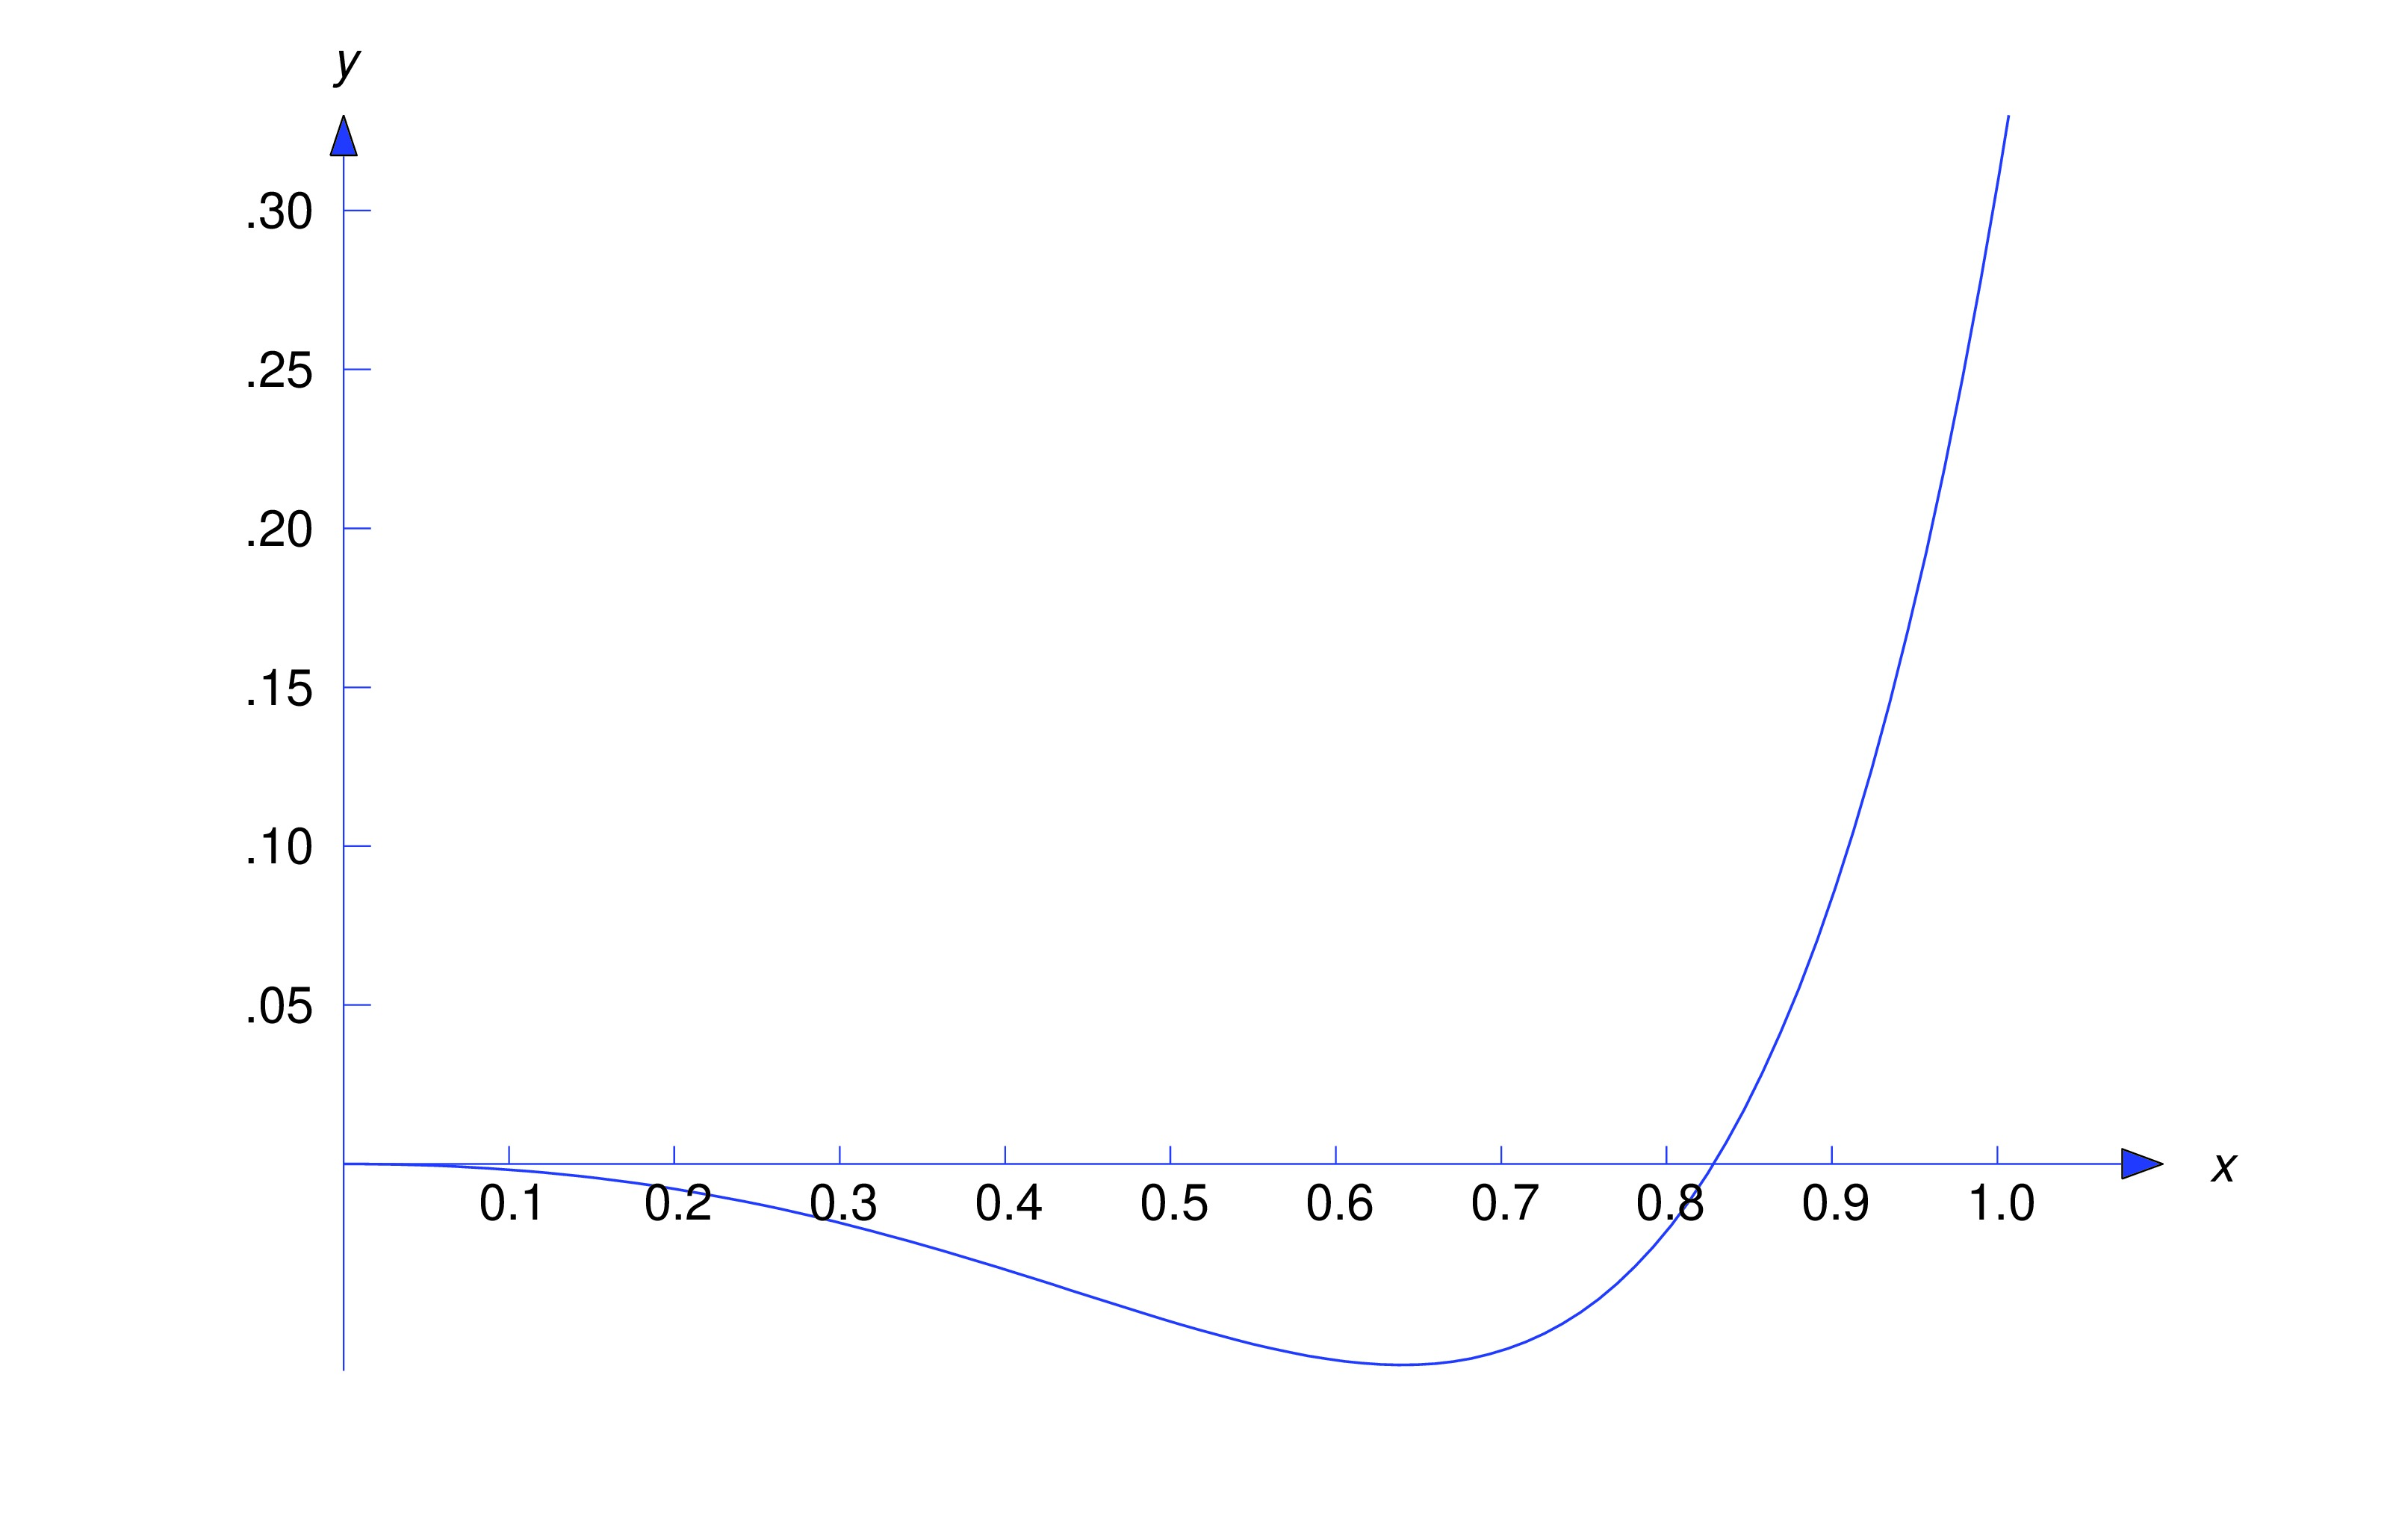
\includegraphics[height=1.5in]{fig090302.jpg} 
\end{image}

\end{explanation}
\end{example}

\subsection*{Forcing Functions of the Form
$e^{\lambda x}\left(P(x)\cos\omega x+Q(x)\sin\omega x\right)$}

We  now consider equations of the form
$$
a_0y^{(n)}+a_1y^{(n-1)}+\cdots+a_ny=
e^{\lambda x}\left(P(x)\cos\omega x+Q(x)\sin\omega x\right),
$$
where $P$ and $Q$ are polynomials.

\begin{example}\label{example:9.3.3}
Find a particular solution of
\begin{equation} \label{eq:9.3.7}
y'''+y''-4y'-4y=e^x[(5-5x)\cos x+(2+5x)\sin x].
\end{equation}


\begin{explanation}
Substituting
\begin{eqnarray*}
y&=&ue^x,\\ y'&=&e^x(u'+u),\\
y''&=&e^x(u''+2u'+u),\\
y'''&=&e^x(u'''+3u''+3u'+u)
\end{eqnarray*}
into \eqref{eq:9.3.7} and canceling $e^x$ yields
$$
(u'''+3u''+3u'+u)+(u''+2u'+u)-4(u'+u)-4u
=(5-5x)\cos x+(2+5x)\sin x,
$$
or
\begin{equation} \label{eq:9.3.8}
u'''+4u''+u'-6u=(5-5x)\cos x+(2+5x)\sin x.
\end{equation}
Since $\cos x$ and $\sin x$ are not solutions of the complementary
equation
$$
u'''+4u''+u'-6u=0,
$$
a theorem analogous to Theorem~\ref{thmtype:5.5.1} implies that
\eqref{eq:9.3.8} has a particular solution of the form
\begin{equation} \label{eq:9.3.9}
u_p=(A_0+A_1x)\cos x+(B_0+B_1x)\sin x.
\end{equation}
Then
\begin{eqnarray*}
u_p'=(A_1+B_0+B_1x)\cos x+(B_1-A_0-A_1x)\sin x,\\
 u_p''=(2B_1-A_0-A_1x)\cos x-(2A_1+B_0+B_1x)\sin x,\\
 u_p'''=-(3A_1+B_0+B_1x)\cos x-(3B_1-A_0-A_1x)\sin x,\\
\end{eqnarray*}
so
$$
\begin{array}{rcl}
u_p'''+4u_p''+u_p'-6u_p&=&-\left[10A_0+2A_1-8B_1+10A_1x\right]\cos
x\\ &&- \left[10B_0+2B_1+8A_1+10B_1x\right]\sin x.
\end{array}
$$
Comparing the coefficients of $x\cos x$, $x\sin x$, $\cos x$, and
$\sin x$ here with the corresponding coefficients in \eqref{eq:9.3.8}
shows that $u_p$ is a solution of \eqref{eq:9.3.8} if
$$
\begin{array}{rcr}
-10A_1&=&-5\\
-10B_1&=&5\\
-10A_0-2A_1+8B_1&=&5\\
-10B_0-2B_1-8A_1&=&2.
\end{array}
$$
Solving the first two equations yields $A_1=1/2$, $B_1=-1/2$.
Substituting these into the last two equations  yields
\begin{eqnarray*}
-10A_0&=&5+2A_1-8B_1=10\\
-10B_0&=&2+2B_1+8A_1=5,
 \end{eqnarray*}
so $A_0=-1$, $B_0=-1/2$.
Substituting $A_0=-1$, $A_1=1/2$, $B_0=-1/2$, $B_1=-1/2$ into
\eqref{eq:9.3.9} shows that
$$
u_p=-\frac{1}{2}\left[(2-x)\cos
x+(1+x)\sin x\right]
$$
is a particular solution of  \eqref{eq:9.3.8}, so
$$
y_p=e^xu_p=-\frac{e^x}{2}\left[(2-x)\cos x+(1+x)\sin x\right]
$$
is a particular  solution of \eqref{eq:9.3.7}.

\begin{image}
 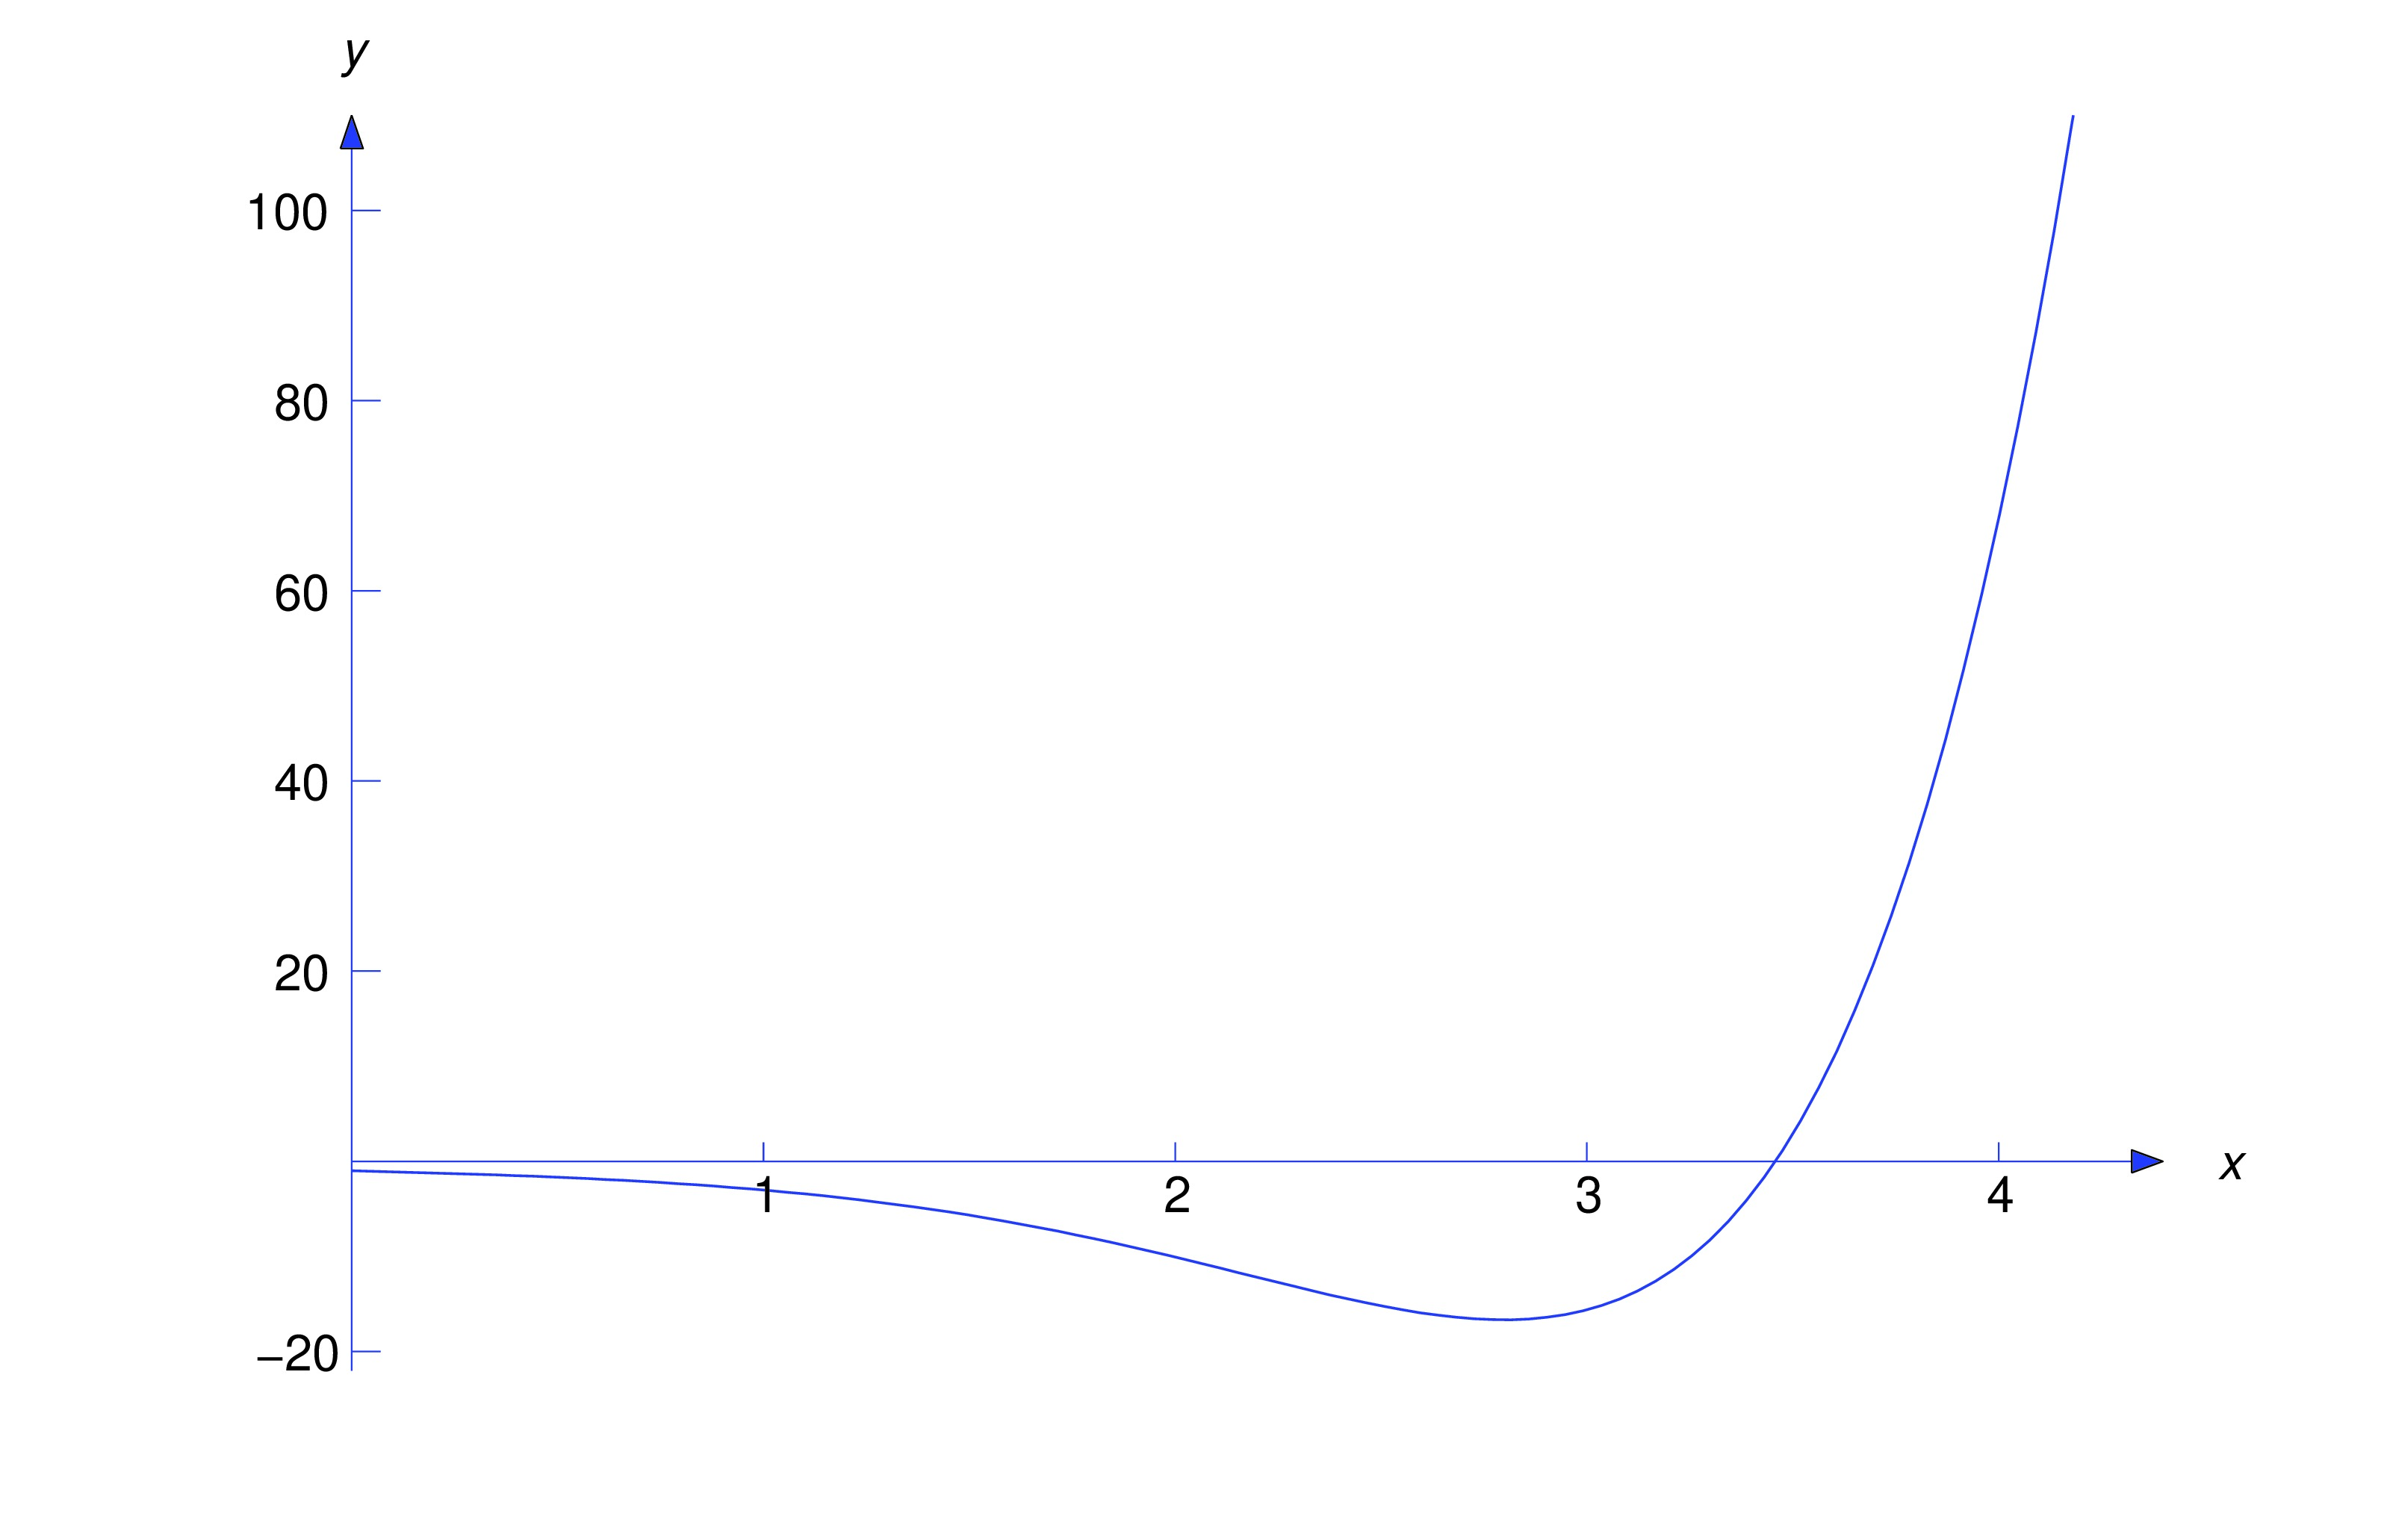
\includegraphics[height=1.5in]{fig090303.jpg} 
\end{image}

     
\end{explanation}
\end{example}




\begin{example}\label{example:9.3.4}
Find a particular solution of
\begin{equation} \label{eq:9.3.10}
 y'''+4y''+6y'+4y=
e^{-x}\left[(1-6x)\cos x-(3+2x)\sin x\right].
\end{equation}

\begin{explanation} 
Substituting
\begin{eqnarray*}
y&=&ue^{-x},\\ y'&=&e^{-x}(u'-u),\\
y''&=&e^{-x}(u''-2u'+u),\\
y'''&=&e^{-x}(u'''-3u''+3u'-u)
\end{eqnarray*}
into \eqref{eq:9.3.10} and canceling $e^{-x}$ yields
$$
(u'''-3u''+3u'-u)+4(u''-2u'+u)+6(u'-u)+4u
=(1-6x)\cos x-(3+2x)\sin x,
$$
or
\begin{equation} \label{eq:9.3.11}
u'''+u''+u'+u=(1-6x)\cos x-(3+2x)\sin x.
\end{equation}
Since $\cos x$ and $\sin x$ are  solutions of the complementary
equation
$$
u'''+u''+u'+u=0,
$$
a theorem analogous to Theorem~\ref{thmtype:5.5.1} implies
that  \eqref{eq:9.3.11} has a particular solution of the form
\begin{equation} \label{eq:9.3.12}
u_p=(A_0x+A_1x^2)\cos x+(B_0x+B_1x^2)\sin x.
\end{equation}

Then
\begin{eqnarray*}
 u_p'&=&[A_0+(2A_1+B_0)x+B_1x^2]\cos
x+[B_0+(2B_1-A_0)x-A_1x^2]\sin x,\\
 u_p''&=&[2A_1+2B_0-(A_0-4B_1)x-A_1x^2]\cos x\\&&+
[2B_1-2A_0-(B_0+4A_1)x-B_1x^2]\sin x,\\
u_p'''&=&-[3A_0-6B_1+(6A_1+B_0)x+B_1x^2]\cos x
\\&&-[3B_0+6A_1+(6B_1-A_0)x-A_1x^2]\sin x,
\end{eqnarray*}
so
$$
\begin{array}{rcl}
u_p'''+u_p''+u_p'+u_p&=&
-[2A_0-2B_0-2A_1-6B_1+(4A_1-4B_1)x]\cos x\\
&&-[2B_0+2A_0-2B_1+6A_1+(4B_1+4A_1)x]\sin x.
\end{array}
$$
Comparing the coefficients of $x\cos x$, $x\sin x$, $\cos x$, and
$\sin x$ here with the corresponding coefficients in \eqref{eq:9.3.11}
shows that $u_p$ is a solution of \eqref{eq:9.3.11} if
$$
\begin{array}{rcr}
-4A_1+4B_1&=&-6\\
-4A_1-4B_1&=&-2\\
-2A_0+2B_0+2A_1+6B_1&=&1\\
-2A_0-2B_0-6A_1+2B_1&=&-3.
\end{array}
$$
Solving the first two equations yields $A_1=1$, $B_1=-1/2$.
Substituting these into the last two equations  yields
\begin{eqnarray*}
-2A_0+2B_0&=&1-2A_1-6B_1=2\\
-2A_0-2B_0&=&-3+6A_1-2B_1=4,
 \end{eqnarray*}

so $A_0=-3/2$ and $B_0=-1/2$.
Substituting $A_0=-3/2$, $A_1=1$, $B_0=-1/2$, $B_1=-1/2$ into
\eqref{eq:9.3.12} shows that
$$
u_p=-\frac{x}{2}\left[(3-2x)\cos
x+(1+x)\sin x\right]
$$
is a particular solution of  \eqref{eq:9.3.11}, so
$$
 y_p=e^{-x}u_p=-\frac{xe^{-x}}{2}\left[(3-2x)\cos
x+(1+x)\sin x\right]
$$
The figure below shows a particular  solution of \eqref{eq:9.3.10}.
\begin{image}
 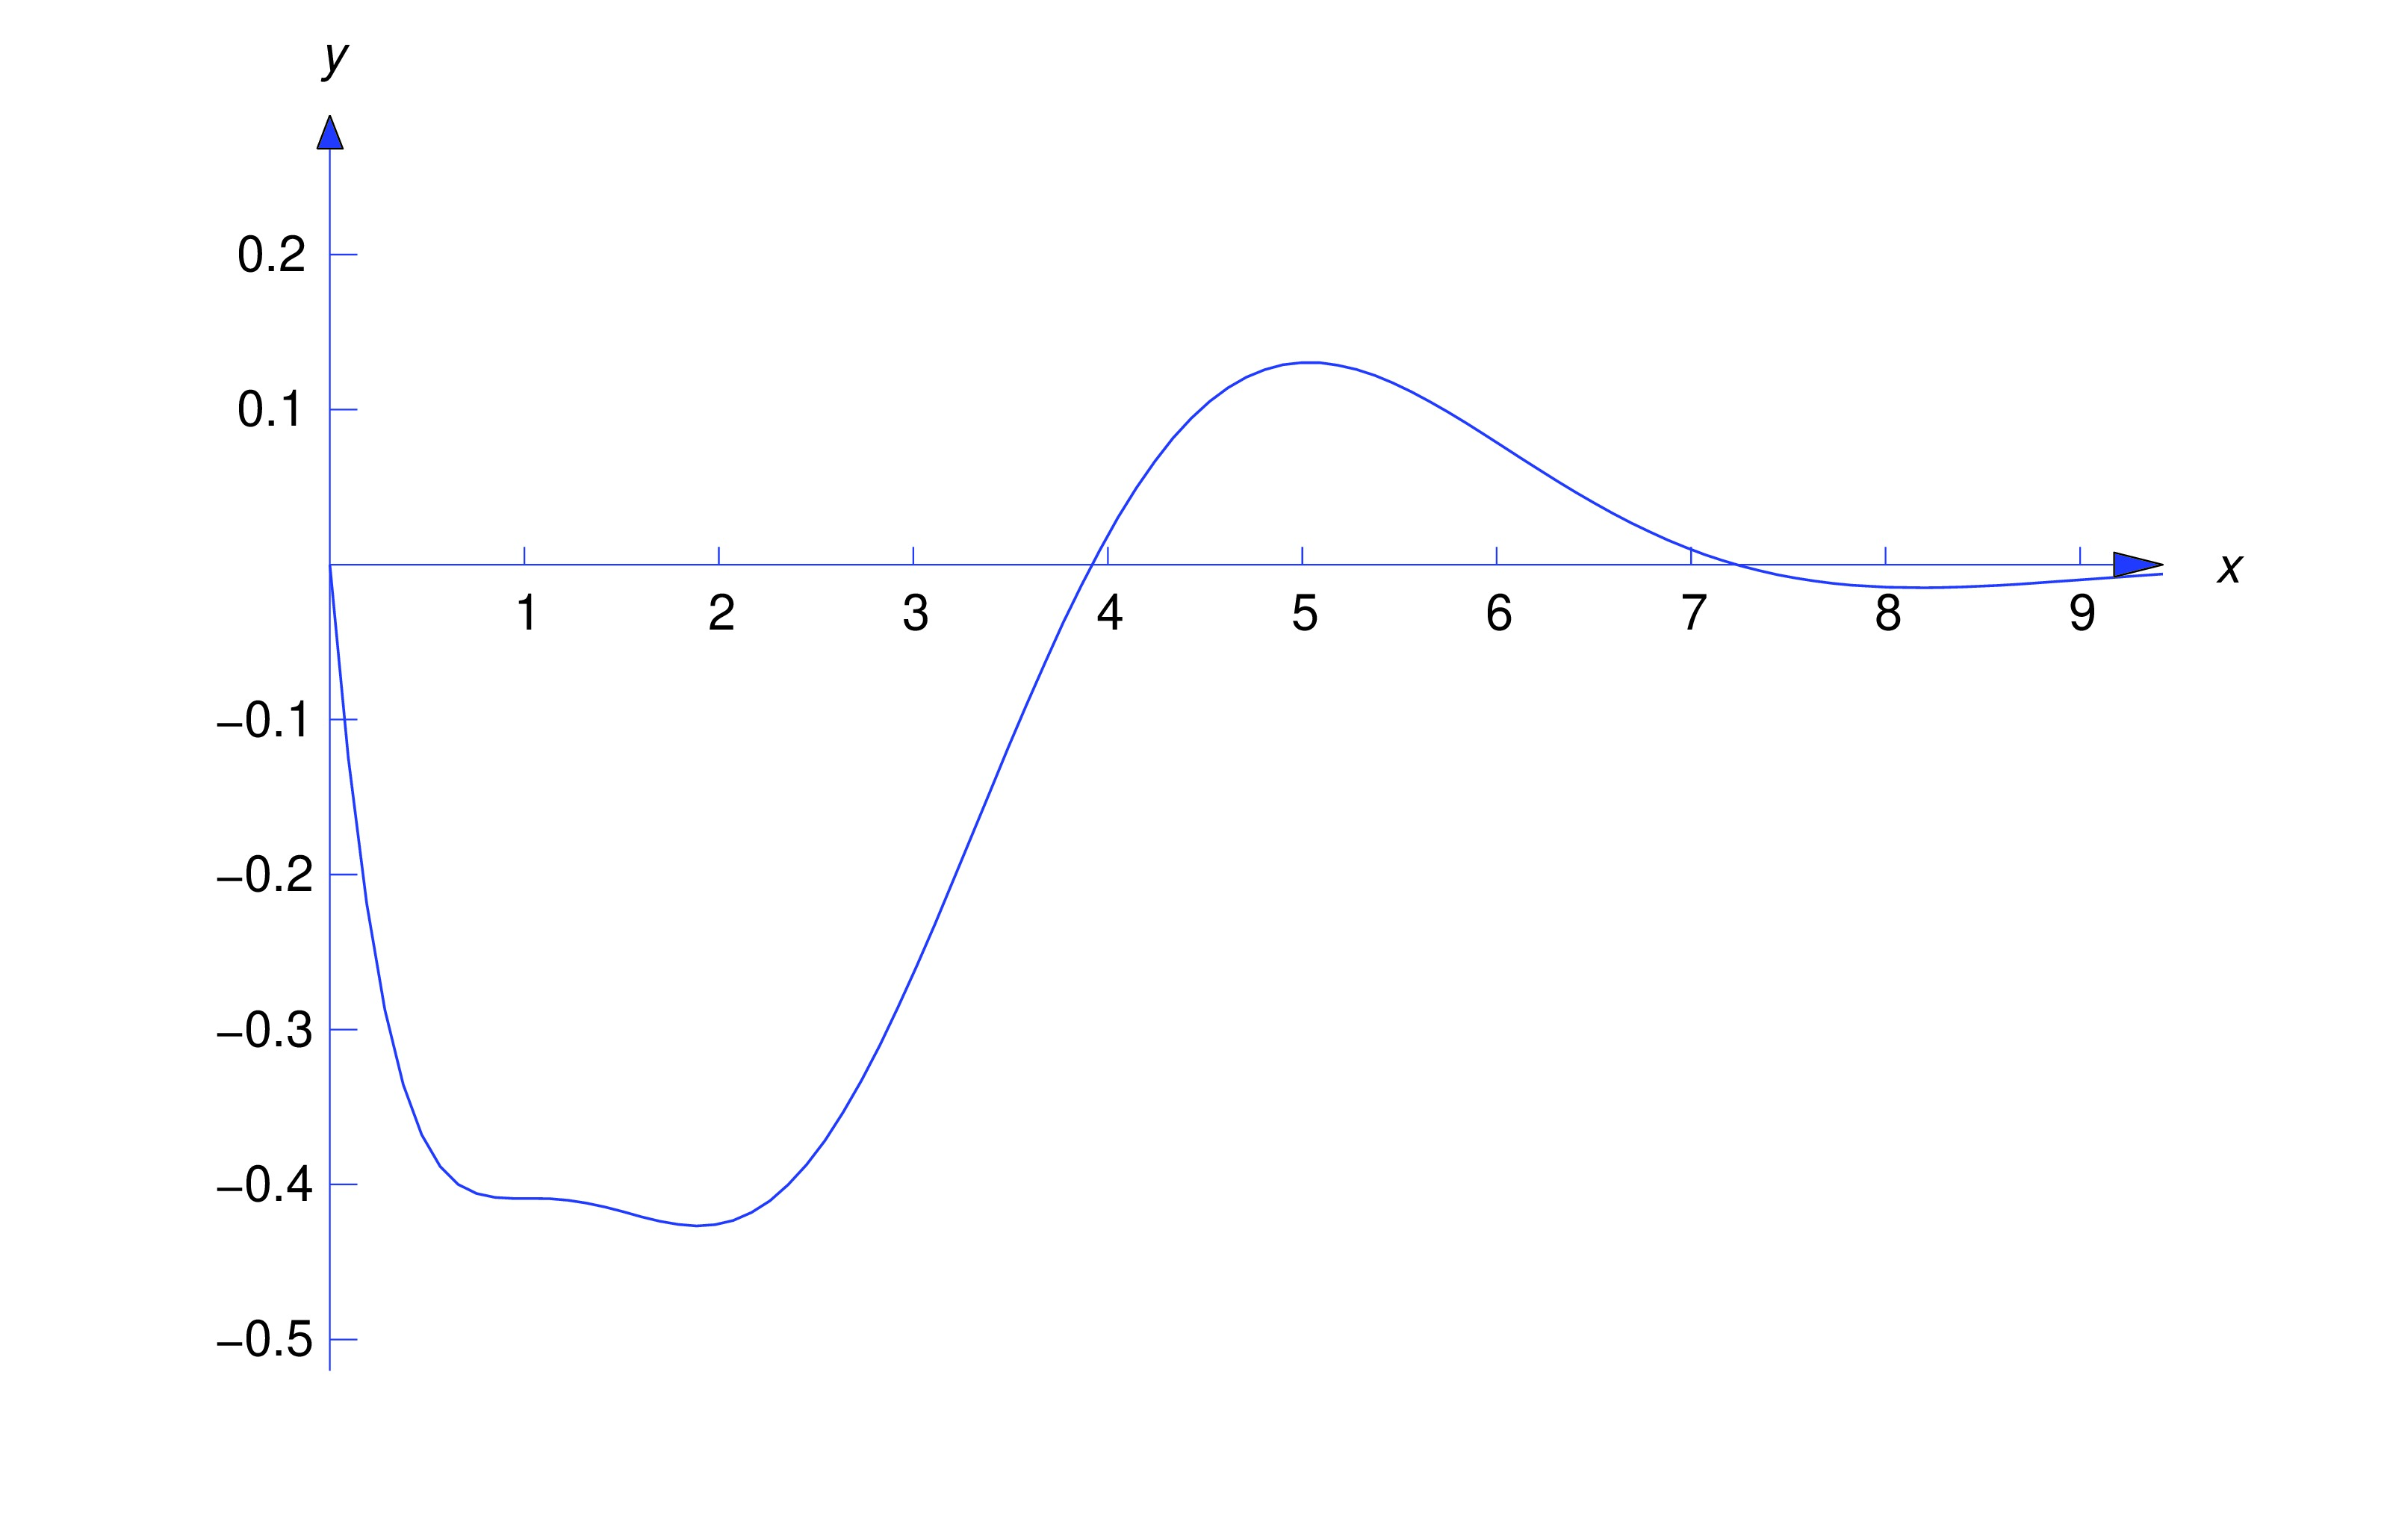
\includegraphics[height=1.5in]{fig090304.jpg} 
\end{image}

\end{explanation}
\end{example}


\section*{Text Source}
Trench, William F., "Elementary Differential Equations" (2013). Faculty Authored and Edited Books \& CDs. 8. (CC-BY-NC-SA)

\href{https://digitalcommons.trinity.edu/mono/8/}{https://digitalcommons.trinity.edu/mono/8/}


\end{document}